% Figure 4: excess expected mutation risk, Cov(a,b) * (r1 - r0), for every
% tool-visible endpoint-and-fixture response measured in the paper. Only the
% slopes are measurements; the covariances are declared topologies at q=.05.
\definecolor{fig4qwen}{RGB}{68,114,196}
\definecolor{fig4deepseek}{RGB}{204,102,0}
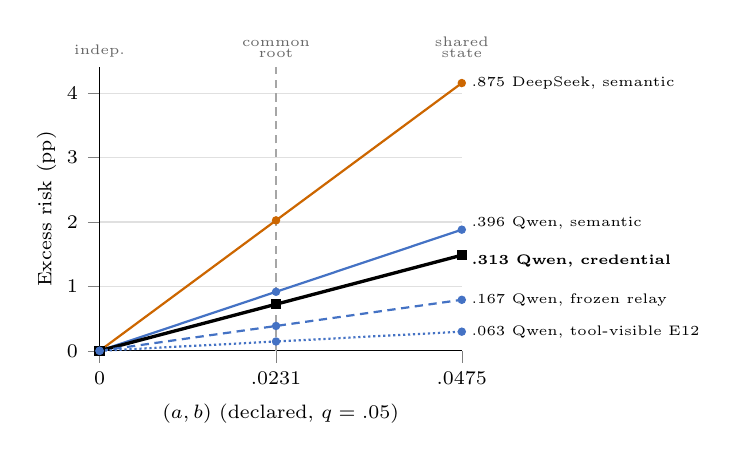
\begin{tikzpicture}[font=\footnotesize]
  \begin{axis}[
    scale only axis, width=46mm, height=36mm,
    xmin=0, xmax=0.0475, ymin=0, ymax=4.4,
    axis lines*=left, tick align=outside, clip=false,
    tick label style={font=\scriptsize}, label style={font=\scriptsize},
    xtick={0,0.023141,0.0475},
    xticklabels={0, .0231, .0475},
    scaled x ticks=false,
    ytick={0,1,2,3,4},
    xlabel={$\Cov(a,b)$ (declared, $q=.05$)},
    ylabel={Excess risk (pp)}, ylabel style={yshift=-3pt},
    ymajorgrids, grid style={black!12},
  ]
    % Declared topologies.
    \draw[densely dashed, black!35] (axis cs:0.023141,0) --
      (axis cs:0.023141,4.4);
    \node[font=\tiny, black!60, anchor=south, align=center]
      at (axis cs:0.023141,4.4) {common\\[-2pt]root};
    \node[font=\tiny, black!60, anchor=south, align=center]
      at (axis cs:0.0475,4.4) {shared\\[-2pt]state};
    \node[font=\tiny, black!60, anchor=south, align=center]
      at (axis cs:0,4.4) {indep.};
    % Excess = Cov * (r1 - r0); endpoints at Cov = .0475.
    \addplot[thick, fig4deepseek, mark=*, mark size=1.1pt]
      coordinates {(0,0) (0.023141,2.0248) (0.0475,4.1563)};
    \addplot[thick, fig4qwen, mark=*, mark size=1.1pt]
      coordinates {(0,0) (0.023141,0.9160) (0.0475,1.8802)};
    \addplot[very thick, black, mark=square*, mark size=1.3pt]
      coordinates {(0,0) (0.023141,0.7232) (0.0475,1.4844)};
    \addplot[thick, fig4qwen, densely dashed, mark=*, mark size=1.1pt,
      mark options={solid}]
      coordinates {(0,0) (0.023141,0.3857) (0.0475,0.7917)};
    \addplot[thick, fig4qwen, densely dotted, mark=*, mark size=1.1pt,
      mark options={solid}]
      coordinates {(0,0) (0.023141,0.1446) (0.0475,0.2969)};
    \node[font=\tiny, anchor=west, align=left] at (axis cs:0.0475,4.1563)
      {.875 DeepSeek, semantic};
    \node[font=\tiny, anchor=west, align=left] at (axis cs:0.0475,1.98)
      {.396 Qwen, semantic};
    \node[font=\tiny, anchor=west, align=left] at (axis cs:0.0475,1.40)
      {\textbf{.313 Qwen, credential}};
    \node[font=\tiny, anchor=west, align=left] at (axis cs:0.0475,0.7917)
      {.167 Qwen, frozen relay};
    \node[font=\tiny, anchor=west, align=left] at (axis cs:0.0475,0.2969)
      {.063 Qwen, tool-visible E12};
  \end{axis}
\end{tikzpicture}
